% TeX root = main.tex

% First argument to \section is the title that will go in the table of contents. Second argument is the title that will be printed on the page.
\section[Lecture 2--{Curves}]{2. Curves}

\subsection{Regular Curves}
\begin{definition}[Regular curve]
    A parameterized curve $c: [a, b] \rightarrow M$ is \textbf{regular}
     if its velocity $c'(t)\neq 0$ for all $t$ in $[a, b]$, which means an immersion from
     $[a, b]$ to $M$.
\end{definition}
\begin{example}
    The curve $c(t)=(t^3, t^2), t\in [-1, 1]$ in $\sR^2$ is not regular since $c'(t)$ is zero
    at $t=0$. 
    Although $c$ is smooth, but the image of $c$ is not smooth as shown 
    in Figure~\ref{fig. t3t2 image}.
\end{example}
\begin{figure}[htb]
    \centering
    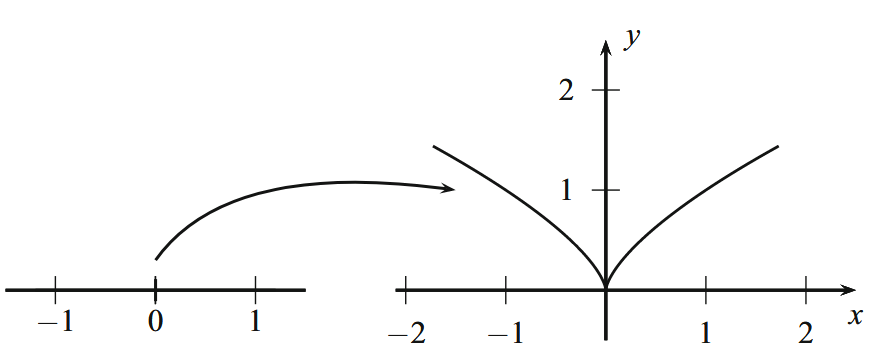
\includegraphics[width=0.7\textwidth]{../Lectures/Figures/image.png}
    \caption{A nonregular curve.}
    \label{fig. t3t2 image}
\end{figure}
\subsection{Arc Length Parameterization}
The most important \textbf{reparameterization} ($\beta(u):=c(t(u))$ if $t=t(u)$ 
is a diffeomorphism from one to another closed interval) 
is the \textbf{arc length reparameterization}.
We define the \textbf{speed} of a curve $c: [a,b]\rightarrow M$ is $\norm{c'(t)}$, and the
arc length is
\begin{align}
    \ell = \int_{a}^{b} \norm{c'(t)}dt. \nonumber
\end{align}
Then, the \textbf{arc length function} $s: [a, b] \rightarrow [0, \ell]$ of $c$ is
\begin{align}
    s(t)=\int_{a}^{t} \norm{c'(t)}dt. \nonumber
\end{align}
\begin{proposition}
    The arc length function $s$ of a regular curve has a $C^\infty$ inverse.
\end{proposition}
\begin{proof}
    The regular property gaurantees $s'(t)=\norm{c'(t)} > 0$, which means $s(t)$ 
    is monotonically increasing, so $t(s)$ is a $C^\infty$ function.
\end{proof}
Thus, we can write the \textbf{arc length reparameterization} of a regular curve
 by $\gamma(s)=c(t(s))$.
\begin{proposition}
    A curve $\gamma(s)$ is reparameterized by arc length if and only if it has \textbf{unit speed} and
    its parameter starts at $0$.
\end{proposition}
\begin{proof}
    $(\Rightarrow)$: as $\gamma(s)=c(t(s))$, the speed is
    \begin{align}
        \norm{\frac{d\gamma}{ds}} = \norm{\frac{dc}{dt}} |\frac{dt}{ds}|
        =\frac{ds}{dt} |\frac{dt}{ds}|=1.
    \end{align}
$(\Leftarrow)$: If $c(t): [a, b]\rightarrow M$ has unit speed that $\norm{c'(t)}=1$,
 the arc length fucntion $s(t)=\int_{a}^{t}dt=t-a$. Since $a=0$, we have $s=t$. Thus, a unit speed curve
 starts at $t=0$ is reparameterized by arc length.
\end{proof}
Here, we do not emphasize that the curve need to be regular since 
\textbf{``reparameterized by arc length'' implies regularity}. The parameter is $s$ or $t$ depends on the
way of reparameterization.
\begin{example}
    The regular curve $c: [0, 2\pi] \rightarrow \sR^2$,
    \begin{align}
        c(t)=(a\cos t, a\sin t), \quad a > 0, \nonumber
    \end{align}
    is a circle of radius $a$ centered at the origin. The arc length function is
    \begin{align}
        s(t) = \int_{0}^{t} \norm{c'(t)} = at. \nonumber
    \end{align}
    So the reparameterization is
    \begin{align}
        \gamma(s) = (a \cos \frac{s}{a}, a \sin \frac{s}{a}). \nonumber
    \end{align}
\end{example}
\subsection{Signed Curvature of a Plane Curve}

\subsection{Orientation and Curvature}

\problemsection{Problems}